% Options for packages loaded elsewhere
\PassOptionsToPackage{unicode,linktoc=all}{hyperref}
\PassOptionsToPackage{hyphens}{url}
\PassOptionsToPackage{dvipsnames,svgnames,x11names}{xcolor}
%
\documentclass[
  a4paper,
]{article}
\usepackage{amsmath,amssymb}
\usepackage{iftex}
\ifPDFTeX
  \usepackage[T1]{fontenc}
  \usepackage[utf8]{inputenc}
  \usepackage{textcomp} % provide euro and other symbols
\else % if luatex or xetex
  \usepackage{unicode-math} % this also loads fontspec
  \defaultfontfeatures{Scale=MatchLowercase}
  \defaultfontfeatures[\rmfamily]{Ligatures=TeX,Scale=1}
\fi
\usepackage{lmodern}
\ifPDFTeX\else
  % xetex/luatex font selection
\fi
% Use upquote if available, for straight quotes in verbatim environments
\IfFileExists{upquote.sty}{\usepackage{upquote}}{}
\IfFileExists{microtype.sty}{% use microtype if available
  \usepackage[]{microtype}
  \UseMicrotypeSet[protrusion]{basicmath} % disable protrusion for tt fonts
}{}
\makeatletter
\@ifundefined{KOMAClassName}{% if non-KOMA class
  \IfFileExists{parskip.sty}{%
    \usepackage{parskip}
  }{% else
    \setlength{\parindent}{0pt}
    \setlength{\parskip}{6pt plus 2pt minus 1pt}}
}{% if KOMA class
  \KOMAoptions{parskip=half}}
\makeatother
\usepackage{xcolor}
\usepackage[margin=25mm]{geometry}
\usepackage{longtable,booktabs,array}
\usepackage{calc} % for calculating minipage widths
% Correct order of tables after \paragraph or \subparagraph
\usepackage{etoolbox}
\makeatletter
\patchcmd\longtable{\par}{\if@noskipsec\mbox{}\fi\par}{}{}
\makeatother
% Allow footnotes in longtable head/foot
\IfFileExists{footnotehyper.sty}{\usepackage{footnotehyper}}{\usepackage{footnote}}
\makesavenoteenv{longtable}
\usepackage{graphicx}
\makeatletter
\def\maxwidth{\ifdim\Gin@nat@width>\linewidth\linewidth\else\Gin@nat@width\fi}
\def\maxheight{\ifdim\Gin@nat@height>\textheight\textheight\else\Gin@nat@height\fi}
\makeatother
% Scale images if necessary, so that they will not overflow the page
% margins by default, and it is still possible to overwrite the defaults
% using explicit options in \includegraphics[width, height, ...]{}
\setkeys{Gin}{width=\maxwidth,height=\maxheight,keepaspectratio}
% Set default figure placement to htbp
\makeatletter
\def\fps@figure{htbp}
\makeatother
\usepackage{svg}
\setlength{\emergencystretch}{3em} % prevent overfull lines
\providecommand{\tightlist}{%
  \setlength{\itemsep}{0pt}\setlength{\parskip}{0pt}}
\setcounter{secnumdepth}{-\maxdimen} % remove section numbering
% definitions for citeproc citations
\NewDocumentCommand\citeproctext{}{}
\NewDocumentCommand\citeproc{mm}{%
  \begingroup\def\citeproctext{#2}\cite{#1}\endgroup}
\makeatletter
 % allow citations to break across lines
 \let\@cite@ofmt\@firstofone
 % avoid brackets around text for \cite:
 \def\@biblabel#1{}
 \def\@cite#1#2{{#1\if@tempswa , #2\fi}}
\makeatother
\newlength{\cslhangindent}
\setlength{\cslhangindent}{1.5em}
\newlength{\csllabelwidth}
\setlength{\csllabelwidth}{3em}
\newenvironment{CSLReferences}[2] % #1 hanging-indent, #2 entry-spacing
 {\begin{list}{}{%
  \setlength{\itemindent}{0pt}
  \setlength{\leftmargin}{0pt}
  \setlength{\parsep}{0pt}
  % turn on hanging indent if param 1 is 1
  \ifodd #1
   \setlength{\leftmargin}{\cslhangindent}
   \setlength{\itemindent}{-1\cslhangindent}
  \fi
  % set entry spacing
  \setlength{\itemsep}{#2\baselineskip}}}
 {\end{list}}
\usepackage{calc}
\newcommand{\CSLBlock}[1]{\hfill\break#1\hfill\break}
\newcommand{\CSLLeftMargin}[1]{\parbox[t]{\csllabelwidth}{\strut#1\strut}}
\newcommand{\CSLRightInline}[1]{\parbox[t]{\linewidth - \csllabelwidth}{\strut#1\strut}}
\newcommand{\CSLIndent}[1]{\hspace{\cslhangindent}#1}
\ifLuaTeX
\usepackage[bidi=basic]{babel}
\else
\usepackage[bidi=default]{babel}
\fi
\babelprovide[main,import]{british}
% get rid of language-specific shorthands (see #6817):
\let\LanguageShortHands\languageshorthands
\def\languageshorthands#1{}
% $HOME/.pandoc/defaults/latex-header-includes.tex
% Common header includes for both lualatex and xelatex engines.
%
% Preliminaries
%
% \PassOptionsToPackage{rgb,dvipsnames,svgnames}{xcolor}
% \PassOptionsToPackage{main=british}{babel}
\PassOptionsToPackage{english}{selnolig}
\AtBeginEnvironment{quote}{\small}
\AtBeginEnvironment{quotation}{\small}
\AtBeginEnvironment{longtable}{\centering}
%
% Packages that are useful to include
%
\usepackage{graphicx}
\usepackage{subcaption}
\usepackage[inkscapeversion=1]{svg}
\usepackage[defaultlines=4,all]{nowidow}
\usepackage{etoolbox}
\usepackage{fontsize}
\usepackage{newunicodechar}
\usepackage{pdflscape}
\usepackage{fnpct}
\usepackage{parskip}
  \setlength{\parindent}{0pt}
\usepackage[style=american]{csquotes}
% \usepackage{setspace} Use the <fontname-plus.tex> files for setspace
%
\usepackage{hyperref} % cleveref must come AFTER hyperref
\usepackage[capitalize,noabbrev]{cleveref} % Must come after hyperref
\let\longdivision\relax
\usepackage{longdivision}
% noto-plus.tex
% Font-setting header file for use with Pandoc Markdown
% to generate PDF via LuaLaTeX.
% The main font is Noto Serif.
% Other main fonts are also available in appropriately named file.
\usepackage{fontspec}
\usepackage{setspace}
\setstretch{1.3}
%
\defaultfontfeatures{Ligatures=TeX,Scale=MatchLowercase,Renderer=Node} % at the start always
%
% For English
% See also https://tex.stackexchange.com/questions/574047/lualatex-amsthm-polyglossia-charissil-error
% We use Node as Renderer for the Latin Font and Greek Font and HarfBuzz as renderer ofr Indic fonts.
%
\babelfont{rm}[Script=Latin,Scale=1]{NotoSerif}% Config is at $HOME/texmf/tex/latex/NotoSerif.fontspec
\babelfont{sf}[Script=Latin]{SourceSansPro}% Config is at $HOME/texmf/tex/latex/SourceSansPro.fontspec
\babelfont{tt}[Script=Latin]{FiraMono}% Config is at $HOME/texmf/tex/latex/FiraMono.fontspec
%
% Sanskrit, Tamil, and Greek fonts
%
\babelprovide[import, onchar=ids fonts]{sanskrit}
\babelprovide[import, onchar=ids fonts]{tamil}
\babelprovide[import, onchar=ids fonts]{greek}
%
\babelfont[sanskrit]{rm}[Scale=1.1,Renderer=HarfBuzz,Script=Devanagari]{NotoSerifDevanagari}
\babelfont[sanskrit]{sf}[Scale=1.1,Renderer=HarfBuzz,Script=Devanagari]{NotoSansDevanagari}
\babelfont[tamil]{rm}[Renderer=HarfBuzz,Script=Tamil]{NotoSerifTamil}
\babelfont[tamil]{sf}[Renderer=HarfBuzz,Script=Tamil]{NotoSansTamil}
\babelfont[greek]{rm}[Script=Greek]{GentiumBookPlus}
%
% Math font
%
\usepackage{unicode-math} % seems not to hurt % fallabck
\setmathfont[bold-style=TeX]{STIX Two Math}
\usepackage{amsmath}
\usepackage{esdiff} % for derivative symbols
% \renewcommand{\mathbf}{\symbf}
%
%
% Other fonts
%
\newfontfamily{\emojifont}{Symbola}
%

\usepackage{titling}
\usepackage{fancyhdr}
    \pagestyle{fancy}
    \fancyhead{}
    \fancyfoot{}
    \renewcommand{\headrulewidth}{0.2pt}
    \renewcommand{\footrulewidth}{0.2pt}
    \fancyhead[LO,RE]{\scshape\thetitle}
    \fancyfoot[CO,CE]{\footnotesize Copyright © 2006\textendash\the\year, R (Chandra) Chandrasekhar}
    \fancyfoot[RE,RO]{\thepage}
%
\usepackage{newunicodechar}
\newunicodechar{√}{\textsf{√}}
\usepackage {caption}
    \captionsetup{font={sf,stretch=1.4}}
\ifLuaTeX
  \usepackage{selnolig}  % disable illegal ligatures
\fi
\IfFileExists{bookmark.sty}{\usepackage{bookmark}}{\usepackage{hyperref}}
\IfFileExists{xurl.sty}{\usepackage{xurl}}{} % add URL line breaks if available
\urlstyle{sf}
\hypersetup{
  pdftitle={The Pi of Archimedes},
  pdfauthor={R (Chandra) Chandrasekhar},
  pdflang={en-GB},
  colorlinks=true,
  linkcolor={DarkOliveGreen},
  filecolor={Purple},
  citecolor={DarkKhaki},
  urlcolor={Maroon},
  pdfcreator={LaTeX via pandoc}}

\title{The Pi of Archimedes}
\author{R (Chandra) Chandrasekhar}
\date{2004-01-14 | 2024-07-13}

\begin{document}
\maketitle

\thispagestyle{empty}


\begin{quote}
This blog began life more than two decades ago, as part of a series of
lectures I delivered to very bright first-year engineering students at
an Australian university.

The number \(\pi\) (pronounced ``pie'') has been recognized from time
immemorial because its physical significance can be grasped easily: it
is the ratio of the circumference of a circle to its diameter. But who
would have thought that such an innocent ratio would exercise such
endless fascination because of the complexities it enfolds?

Not surprisingly, some high students I met recently wanted to know more
about \(\pi\). Accordingly, I have substantially recast and refreshed my
original presentation to better accord with the form and substance of a
blog. The online references have also been updated to keep up with a
rapidly changing Web.

My original intention was to write a single blog on \(\pi\). But because
I did not want it to become yet another overly long \emph{slog}, I have
decided to divide the material into two parts.

If there are any errors or omissions, please
\href{mailto:feedback.swanlotus@gmail.com}{email} me your feedback.
\end{quote}

\subsection{Circumference, diameter, and
π}\label{circumference-diameter-and-ux3c0}

The straight line or
\href{https://mathworld.wolfram.com/Geodesic.html}{geodesic} is the
shortest distance between any two points on a plane, sphere, or other
space. The circle is the
\href{https://en.wikipedia.org/wiki/Locus_(mathematics)}{locus}
traversed by a moving point that is
\href{https://en.wikipedia.org/wiki/Equidistant}{equidistant} from
another fixed point on a two-dimensional plane. It is the most
\href{https://mathworld.wolfram.com/Symmetry.html}{symmetrical} figure
on the plane. The
\href{https://en.wikipedia.org/wiki/Diameter}{diameter} is the name
given both to any straight line passing through the centre of the
circle---intersecting it at two points---as well as to its length. When
we divide the \href{https://en.wikipedia.org/wiki/Perimeter}{perimeter}
of a circle, more properly called its
\href{https://en.wikipedia.org/wiki/Circumference}{circumference},
\(C\), by its diameter, \(d\), we get the enigmatic constant \(\pi\),
which has a value between \(3.141\) and \(3.142\):
\begin{equation}\phantomsection\label{eq:pi-Cd}{
\frac{C}{d} = \pi.
}\end{equation} The diameter \(d\) is twice the radius \(r\), and
substituting for \(d\) into \cref{eq:pi-Cd}, we get the well-known
school formula: \begin{equation}\phantomsection\label{eq:two-pi-r}{
C = \pi d = 2\pi r \approx 2\left[\frac{22}{7}\right]r \approx 6.28r.
}\end{equation} Note, however, that \(\pi\) is \emph{not exactly equal}
to \(\frac{22}{7}\). This value is a convenient \emph{rational fraction
approximation} for \(\pi\) that serves well in elementary
contexts.\footnote{See
  \href{https://swanlotus.netlify.app/blogs/a-tale-of-two-measures-degrees-and-radians}{``A
  tale of two measures: degrees and radians''}.}

You might reasonably wonder whether the ratio of the circumference to
the diameter of \emph{any} circle is \emph{always} \(\pi\). The answer
is ``Yes'', because \emph{all circles are similar}. The ratios of
corresponding lengths of similar figures are equal. This idea is also
covered in my blog
\href{https://swanlotus.netlify.app/blogs/a-tale-of-two-measures-degrees-and-radians}{``A
tale of two measures: degrees and radians''}.

The symbol \href{https://en.wikipedia.org/wiki/Pi}{\(\pi\)} is the
lowercase version of the sixteenth letter of the Greek alphabet. For the
history of its use in mathematics, see
\href{https://en.wikipedia.org/wiki/Pi\#Adoption_of_the_symbol_\%CF\%80}{adoption
of the symbol π in Wikipedia}.

\begin{figure}
\centering
\includesvg[width=0.7\textwidth,height=\textheight]{images/C-over-d.svg}
\caption{The ratio of the circumference to the diameter of \emph{any}
circle is \(\pi\).}\label{fig:pi-circle}
\end{figure}

\cref{fig:pi-circle} shows the relationships in
\cref{eq:pi-Cd,eq:two-pi-r} pictorially. The circumference of a circle
is about 6.28 times its radius. Why this should be so is a secret of
Nature, a mystery of the space we inhabit.

A wonderfully revealing story lies behind this mysterious relationship,
and it is due to the
\href{https://www.collinsdictionary.com/dictionary/english/labours}{labours}
of one man, in the days when calculators could not be dreamed of, and
when neither the decimal system of numbers, nor trigonometry were known.
That is the story we look at next.

\subsection{Archimedes of Syracuse}\label{archimedes-of-syracuse}

\href{https://en.wikipedia.org/wiki/Archimedes}{Archimedes of
Syracuse}\footnote{His very name, Archimedes, means ``master thinker''
  in Greek.} (Ἀρχιμήδης, 287--212 BCE) was a
\href{https://www.vocabulary.com/dictionary/polymath\#:~:text=Definitions\%20of\%20polymath,of\%20great\%20and\%20varied\%20learning}{polymath}
and genius of the ancient world. He was one of the greatest
mathematicians the world has ever known. By today's standards, he would
be called a mathematician, physicist, engineer, and astronomer,
\href{https://www.ldoceonline.com/dictionary/all-rolled-into-one}{all
rolled into one}. He is perhaps most famous for running out of his
bathtub naked exclaiming
\href{https://www.dictionary.com/browse/eureka}{``Eureka''}---Greek for
``I have found it''---oblivious of those around him. The principle that
he had then discovered---that the upthrust on a body submerged in a
fluid is equal to the weight of fluid displaced---is known as
\href{https://www.britannica.com/science/Archimedes-principle}{Archimedes'
Principle}.

\begin{figure}
\centering
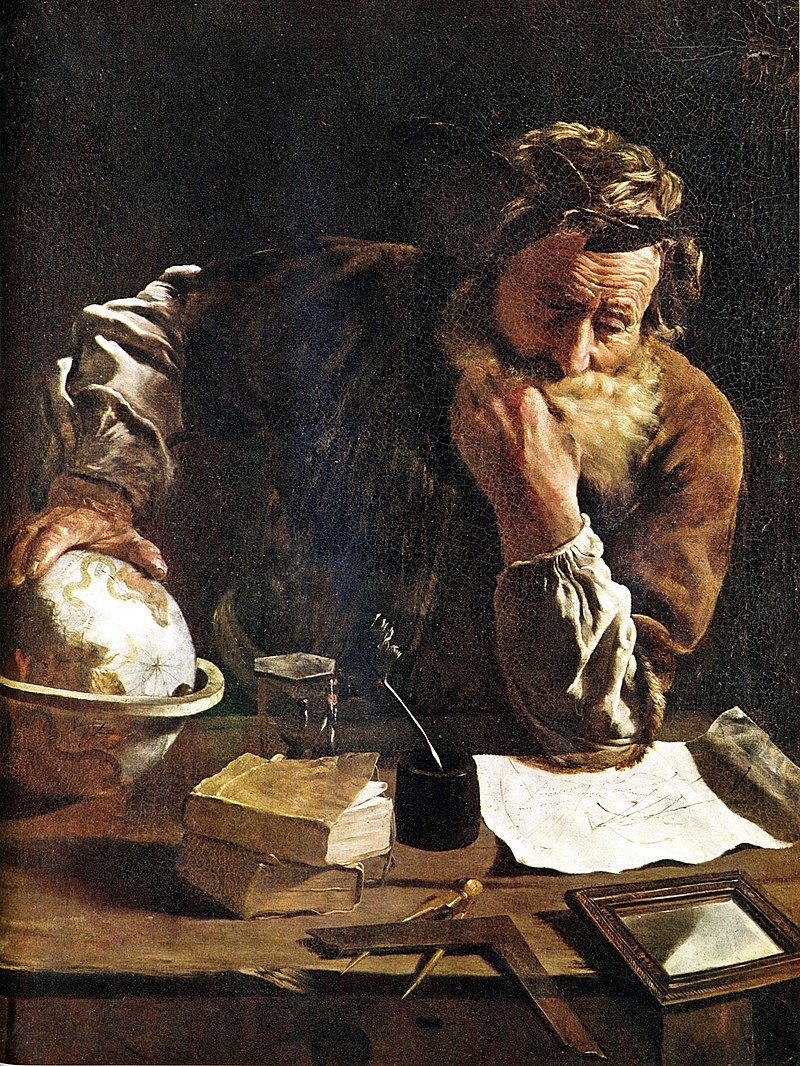
\includegraphics[width=0.5\textwidth,height=\textheight]{images/Domenico-Fetti_Archimedes_1620.jpg}
\caption[Archimedes of Syracuse.]{Archimedes of
Syracuse.\footnotemark{}}\label{fig:archimedes}
\end{figure}
\footnotetext{Domenico Fetti's 1620 painting entitled \emph{Archimedes
  Thoughtful}. Public domain.}

Among the many accomplishments of Archimedes is his method for
estimating \(\pi\), which was the best approximation for almost 1900
years. And it was not based on using a length of string, superimposing
it on a circle, and getting an estimate! \emojifont {😉}\normalfont

What is even more remarkable is that Archimedes made his discovery
\emph{without} the benefit of:

\begin{enumerate}
\def\labelenumi{(\alph{enumi})}
\item
  the real numbers;
\item
  algebra;
\item
  trigonometry;
\item
  decimal notation; and
\item
  devices like logarithm tables, slide rules, calculators, or computers.
\end{enumerate}

Instead he applied geometry---including the theorem of Pythagoras---and
extracted rational values for square roots, laboriously by hand.

His method is also an excellent geometrical illustration of the idea of
a
\href{https://www.britannica.com/science/limit-mathematics}{\emph{limit}},
with which he was doubtless familiar. It is known that Archimedes was
familiar with what we now know as integral calculus, and it is possible
that he may have anticipated differential calculus as well.

Archimedes devised an ingenious method for estimating \(\pi\) by
obtaining successively more accurate values for the circumference of a
circle.

\begin{figure}
\centering
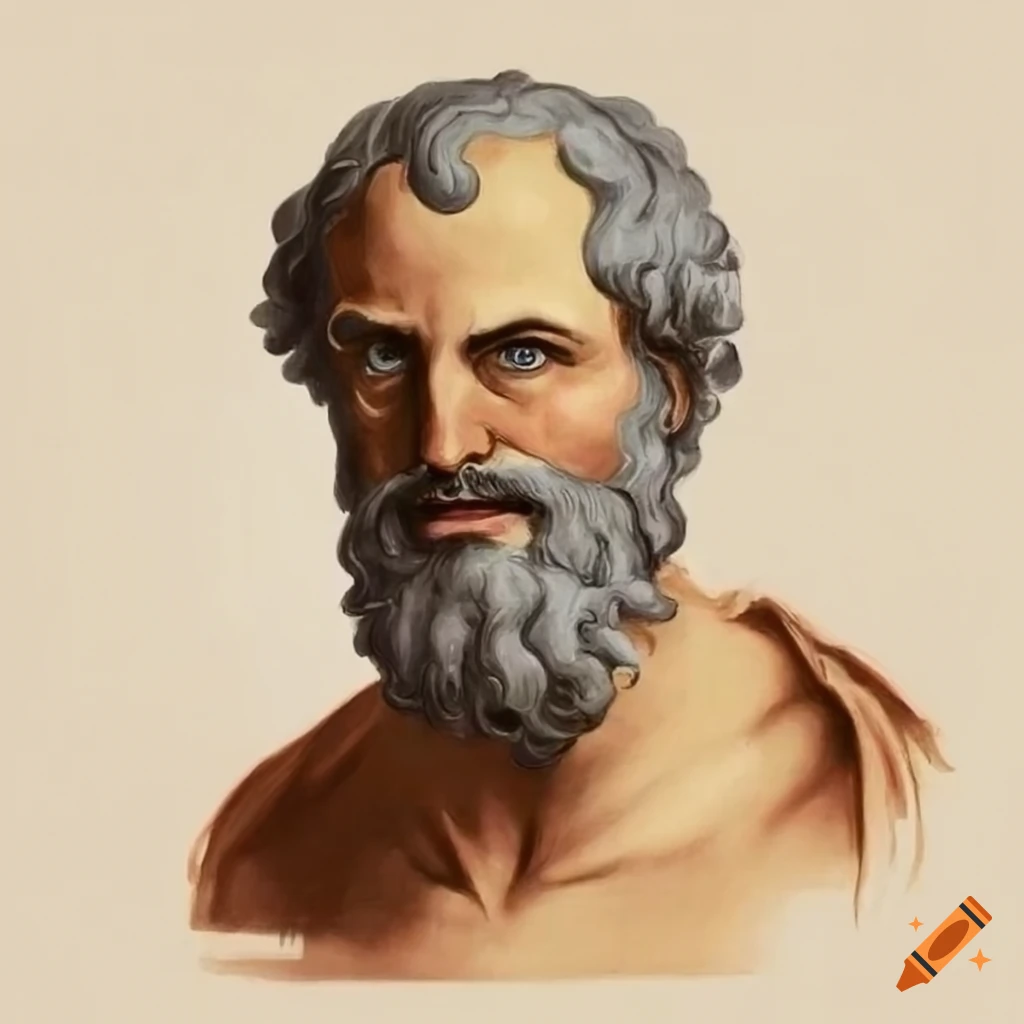
\includegraphics[width=0.7\textwidth,height=\textheight]{images/Archimedes-AI-generated-portrait.png}
\caption{Portrait of Archimedes generated by AI and available at the
Craiyon website
\href{https://www.craiyon.com/image/JEmP4rPCRW25xyCULOeMSw}{here}. All
portraits of Archimedes are flights of fancy rather than true
likenesses.}\label{fig:Archimedes-AI}
\end{figure}

\subsection{Principles used by
Archimedes}\label{principles-used-by-archimedes}

The method that Archimedes devised is instructive because it is a
synthesis of several principles by which the greatest human minds have
furthered scientific progress over time. The abstract principles that
Archimedes used to estimate \(\pi\) include:

\begin{enumerate}
\item
  Start with the known and progress to the unknown;
\item
  Initialize variables;
\item
  Devise a method of increasing the accuracy of the estimate by
  \emph{looping through or repeating the same process};\footnote{These
    are called
    \href{https://mathworld.wolfram.com/Recursion.html}{recursion} or
    \href{https://www.vocabulary.com/dictionary/iteration}{iteration}---as
    the case may be---in computer science.}
\item
  Stop when the desired accuracy is reached.
\end{enumerate}

These steps constitute what is known as an
\href{https://www.merriam-webster.com/dictionary/algorithm}{algorithm}.
Once such a systematic framework has been put in place, it can be
applied in many research domains to aid rapid scientific progress. The
algorithm is the basis of modern computing.

\subsection{Of polygons and circles}\label{of-polygons-and-circles}

Archimedes wanted to estimate the \emph{circumference} and \emph{area of
a circle} by a systematic and logical method. That \(\pi\) is involved
in both of these is somewhat incidental. Nevertheless, his approach is
the first well documented account of how to estimate \(\pi\) with
reasonable accuracy, and is the focus of our blog.

Archimedes considered a circle, containing an
\href{https://mathworld.wolfram.com/Inscribed.html}{inscribed} regular
polygon with \(n\) sides, and
\href{https://mathworld.wolfram.com/Circumscribed.html}{circumscribed}
by a regular polygon with the same \(n\) sides. \cref{fig:two-limits}
illustrates this for the case \(n = 6\), i.e., with a regular
\href{https://www.britannica.com/science/hexagon}{hexagon}.

\begin{figure}
\centering
\includesvg[width=0.7\textwidth,height=\textheight]{images/two-limits.svg}
\caption{The circumference of the circle in darkolivegreen is bounded
from below by the perimeter of the inscribed regular hexagon in maroon
and bounded from above by the perimeter of the circumscribed regular
hexagon in midnightblue. The circumference of the circle must lie
between the perimeters of these two hexagons. The value \(r\) is the
radius of the circle and the height \(h\)---from the centre to the
mid-point of a side---is called the
\href{https://en.wikipedia.org/wiki/Apothem}{apothem}.}\label{fig:two-limits}
\end{figure}

\begin{figure}
\centering
\includesvg[width=0.7\textwidth,height=\textheight]{images/sin-theta-tan-theta.svg}
\caption[The relationship between the circle and its inscribed and
circumscribed regular polygons. The symbol \(h\) is used for the apothem
in both cases. Note that \(OD = h = r\cos\theta\) for the inscribed
polygon, whereas \(OC = h = r\) for the circumscribed polygon.]{The
relationship between the circle and its inscribed and circumscribed
regular polygons. The symbol \(h\) is used for the apothem in both
cases. Note that \(OD = h = r\cos\theta\) for the inscribed polygon,
whereas \(OC = h = r\) for the circumscribed
polygon.\footnotemark{}}\label{fig:sin-theta-tan-theta}
\end{figure}
\footnotetext{Recall that the area of a triangle is half the product of
  its base and perpendicular height}

Let us tabulate below the variables arising from
\cref{fig:two-limits,fig:sin-theta-tan-theta}.

\begin{longtable}[]{@{}
  >{\raggedright\arraybackslash}p{(\columnwidth - 6\tabcolsep) * \real{0.1270}}
  >{\raggedright\arraybackslash}p{(\columnwidth - 6\tabcolsep) * \real{0.1746}}
  >{\raggedright\arraybackslash}p{(\columnwidth - 6\tabcolsep) * \real{0.4127}}
  >{\raggedright\arraybackslash}p{(\columnwidth - 6\tabcolsep) * \real{0.2857}}@{}}
\caption{\label{tbl:variables}Circle, inscribed, and circumscribed
regular polygons (\(n\)-gons).}\tabularnewline
\toprule\noalign{}
\begin{minipage}[b]{\linewidth}\raggedright
Parameter
\end{minipage} & \begin{minipage}[b]{\linewidth}\raggedright
Circle
\end{minipage} & \begin{minipage}[b]{\linewidth}\raggedright
Inscribed
\end{minipage} & \begin{minipage}[b]{\linewidth}\raggedright
Circumscribed
\end{minipage} \\
\midrule\noalign{}
\endfirsthead
\toprule\noalign{}
\begin{minipage}[b]{\linewidth}\raggedright
Parameter
\end{minipage} & \begin{minipage}[b]{\linewidth}\raggedright
Circle
\end{minipage} & \begin{minipage}[b]{\linewidth}\raggedright
Inscribed
\end{minipage} & \begin{minipage}[b]{\linewidth}\raggedright
Circumscribed
\end{minipage} \\
\midrule\noalign{}
\endhead
\bottomrule\noalign{}
\endlastfoot
Radius & \(r\) & & \\
Sides & & \(n\) & \(n\) \\
Length & & \(2r\sin\theta\) & \(2r\tan\theta\) \\
Angle & & \(\theta(n) = \frac{\pi}{n} = \frac{180°}{n}\) &
\(\theta(n) = \frac{\pi}{n}=\frac{180°}{n}\) \\
Apothem & & \(h = r\cos\theta\) & \(h = r\) \\
Area & \(A = \pi r^2\) & \(a(n) = n\sin\theta\cos\theta r^2\) &
\(A(n) = n\tan\theta r^2\) \\
Perimeter & \(C = 2\pi r\) & \(c(n) = 2n\sin\theta r\) &
\(C(n) = 2n\tan\theta r\) \\
\end{longtable}

When \(n\) varies, so do the values of \(\theta\) and the areas and
perimeters; they are therefore shown as functions of \(n\) in
\cref{tbl:variables}.

\subsection{Looping}\label{looping}

Archimedes started with regular hexagons and successively \emph{doubled}
the number of sides, until he had the circle closely sandwiched between
two 96-sided-regular polygons---one inscribed; the other circumscribed.

Successively doubling or halving is a fast-converging technique used in
numerical estimation, called the
\href{https://en.wikipedia.org/wiki/Bisection_method}{bisection method},
that is applied to solving a variety of problems. That Archimedes was
aware of it, shows how far ahead of his time his thinking was.

When he moved from \(n=6\) to \(n = 12\) sides, how did Archimedes
estimate the respective perimeters without the aid of trigonometry? He
used geometry and the Pythagorean theorem,
\href{https://nonagon.org/ExLibris/archimedes-pi}{as described online
here} {[}\citeproc{ref-bertrand2014}{1}{]}
\href{https://publications.azimpremjiuniversity.edu.in/3356/1/02-DaminiAndAbhishek_PiIs22By7_Final.pdf}{and
here} {[}\citeproc{ref-damini-dhar-2020}{2}{]} to obtain
\href{https://en.wikipedia.org/wiki/Recurrence_relation}{recurrence
relations} that gave the current perimeter from the previous one.

For an English translation of the book \emph{Measurement of a Circle} by
Archimedes \href{auxiliary/Archimedes-Circle.pdf}{click on this link}.
It is the original source material from the man himself, and will give
you a sense of completeness in your understanding of his method.

He repeatedly calculated \emph{rational approximations} to \(\pi\) until
he was satisfied with the accuracy. The principle of the method is
clearly illustrated in
\cref{fig:six-gon,fig:twelve-gon,fig:twenty-four-gon,fig:forty-eight-gon,fig:ninety-six-gon}.

\begin{figure}
\centering
\includesvg[width=0.7\textwidth,height=\textheight]{images/six-gon.svg}
\caption{The estimate for \(\pi\) lies between
\(c(6) = 3.0000 < \pi < C(6) = 3.4641\).}\label{fig:six-gon}
\end{figure}

\begin{figure}
\centering
\includesvg[width=0.7\textwidth,height=\textheight]{images/twelve-gon.svg}
\caption{The estimate for \(\pi\) lies between
\(c(12) = 3.1058 < \pi < C(12) = 3.2153\).}\label{fig:twelve-gon}
\end{figure}

\begin{figure}
\centering
\includesvg[width=0.7\textwidth,height=\textheight]{images/twenty-four-gon.svg}
\caption{The estimate for \(\pi\) lies between
\(c(24) = 3.1326 < \pi < C(24) = 3.1596\).}\label{fig:twenty-four-gon}
\end{figure}

\begin{figure}
\centering
\includesvg[width=0.7\textwidth,height=\textheight]{images/forty-eight-gon.svg}
\caption{The estimate for \(\pi\) lies between
\(c(48) = 3.1393 < \pi < C(48) = 3.1460\).}\label{fig:forty-eight-gon}
\end{figure}

\begin{figure}
\centering
\includesvg[width=0.7\textwidth,height=\textheight]{images/ninety-six-gon.svg}
\caption{The estimate for \(\pi\) lies between
\(c(96) = 3.1410 < \pi < C(96) = 3.1427\). Notice in this sequence of
images how the circumference of the circle approaches the perimeter of
the inscribed and circumscribed heaxgons to the point of being
indistinguishable from either of them. \emph{The final estimate of
Archimedes was
\(\frac{223}{71} < \pi < \frac{22}{7}\).}}\label{fig:ninety-six-gon}
\end{figure}

\textbf{The final estimate of Archimedes was
\(\frac{223}{71} < \pi < \frac{22}{7}\).}

\subsection{Calculus before it was
discovered}\label{calculus-before-it-was-discovered}

Evaluating the bounds given in \cref{tbl:variables} and
\cref{eq:squeeze} by setting \(r = 1\), \(n = 6\), and
\(\theta = \frac{180}{n} = 30°\)\footnote{Rather than use radians with
  \(\pi\) entering the proceedings, I decided to stick with degrees as
  units to avoid confusion. If one uses power series to probe further,
  of course, radians are called for.} gives us these values, expressed
to four decimal places:
\begin{equation}\phantomsection\label{eq:triple-6}{
\begin{aligned}
C_i &= 2n\sin\theta r = 12(\sin 30°) = 12(0.5) &= 6.0000.\\
C &= 2\pi r &= 6.2381.\\
C_c &= 2n\tan\theta r = 12(\tan 30°) = 12\left(\tfrac{\sqrt{3}}{3}\right) = 4\sqrt{3} &\approx 6.9282.\\
\end{aligned}
}\end{equation}

Archimedes doubled \(n\) four times to compute values for regular
polygons with \(12\), \(24\), \(48\), and \(96\) sides. For his last
calculation with \(n = 96\) and
\(\theta = \tfrac{180}{96}° \approx 1.875°\), we have:
\begin{equation}\phantomsection\label{eq:triple-96}{
\begin{aligned}
C_i &= 2n\sin\theta r = 2(96)\sin{1.875°} \approx 192(0.0327) &\approx 6.2820.\\
C &= 2\pi r &= 6.2381.\\
C_c &= 2n\tan\theta r = 2(96)\tan{1.875°} \approx 192(0.0327) &\approx 6.2854.\\
\end{aligned}
}\end{equation}

Note that in the case of 96 sides, we have a \emph{very small angle}
\(\theta\) whose \(\sin\) and \(\tan\) are almost equal. This is what
gives us tight bounds on the estimate of \(\pi\). If you know
\href{https://math.libretexts.org/Bookshelves/Differential_Equations/A_First_Course_in_Differential_Equations_for_Scientists_and_Engineers_(Herman)/08:_Appendix_Calculus_Review/8.07:_Power_Series}{the
power series for \(\sin\theta\) and \(\tan\theta\)}, you will appreciate
even better how the value of \(\pi\) is trapped and squeezed between
these two rather close limits.

Remember \cref{eq:triple-96} because it helps us to estimate lower and
upper bounds for the value of the circumference. Archimedes's
application of the
\href{https://en.wikipedia.org/wiki/Squeeze_theorem}{squeeze theorem}
nineteen centuries before the calculus was invented is illustrated in
the series of
\cref{fig:six-gon,fig:twelve-gon,fig:twenty-four-gon,fig:forty-eight-gon,fig:ninety-six-gon}.

If you study the calculus or analysis later on, and encounter the
\href{https://en.wikipedia.org/wiki/Limit_of_a_function}{epsilon-delta
(\(\epsilon-\delta\)) definition of a limit} hark back to this example
of Archimedes for a graphic and concrete example of how a value may be
bounded from below and above and how it may be
\href{https://demonstrations.wolfram.com/SqueezeTheorem/}{squeezed} into
the limit.

\subsection{Conclusions from initial
results}\label{conclusions-from-initial-results}

If we divide the last row of entries in \cref{tbl:variables} by \(2r\),
we get the entries \(\pi\), \(n\sin\theta\), and \(n\tan\theta\). We
will use these values henceforth as they are directly comparable and
relatable to \(\pi\). \begin{equation}\phantomsection\label{eq:squeeze}{
\begin{aligned}
a(n) < A < A(n) &\implies n\sin\theta\cos\theta < \pi < n\tan\theta\\
c(n) < C < C(n) &\implies n\sin\theta < \pi < n\tan\theta\\
\end{aligned}
}\end{equation}

From the right hand side of \cref{eq:squeeze}, using the inequalities
for perimeters, we have
\begin{equation}\phantomsection\label{eq:lower-bound}{
n\sin\tfrac{180°}{n} = n\sin\tfrac{\pi}{n}, \thinspace \mbox{for the lower bound}.
}\end{equation} and
\begin{equation}\phantomsection\label{eq:upper-bound}{
n\tan\tfrac{180°}{n} = n\tan\tfrac{\pi}{n}, \thinspace \mbox{for the upper bound}.
}\end{equation}

\cref{eq:lower-bound,eq:upper-bound} represent respectively the lower
and upper bounds on the value of \(\pi\) obtained through the method of
Archimedes using \emph{polygon perimeter}.

If, instead, we were to use \emph{polygon area}, the relevant equations
will be obtained by dividing the second last row of \cref{tbl:variables}
by \(r^2\). The resulting equations will be:
\begin{equation}\phantomsection\label{eq:area-lower-bound}{
n\sin\tfrac{180°}{n}\cos\tfrac{180°}{n} = n\sin\tfrac{\pi}{n}\cos\tfrac{\pi}{n}, \thinspace \mbox{for the lower bound}.
}\end{equation} and
\begin{equation}\phantomsection\label{eq:area-upper-bound}{
n\tan\tfrac{180°}{n} = n\tan\tfrac{\pi}{n}, \thinspace \mbox{for the upper bound}.
}\end{equation}

Note that \cref{eq:upper-bound} and \cref{eq:area-upper-bound} are
equal. Therefore, the upper bound is the same, regardless of whether we
consider polygon area or perimeter.

Obviously, the circle may be viewed as a regular polygon whose number of
sides, \(n\), has become exceedingly large, or \emph{infinite}. So, as
\(n\) is increased, we should expect the two bounds to converge to the
limiting value of \(\pi\).

\begin{longtable}[]{@{}
  >{\raggedleft\arraybackslash}p{(\columnwidth - 8\tabcolsep) * \real{0.1447}}
  >{\raggedleft\arraybackslash}p{(\columnwidth - 8\tabcolsep) * \real{0.2105}}
  >{\raggedleft\arraybackslash}p{(\columnwidth - 8\tabcolsep) * \real{0.2105}}
  >{\raggedleft\arraybackslash}p{(\columnwidth - 8\tabcolsep) * \real{0.2237}}
  >{\raggedleft\arraybackslash}p{(\columnwidth - 8\tabcolsep) * \real{0.2105}}@{}}
\caption{\label{tbl:large-n-pi}Estimates of \(\pi\) from the perimeters
and areas of inscribed and circumscribed polygons of \(n\)
sides.}\tabularnewline
\toprule\noalign{}
\begin{minipage}[b]{\linewidth}\raggedleft
\(n\)
\end{minipage} & \begin{minipage}[b]{\linewidth}\raggedleft
\(n\sin\frac{180°}{n}\)
\end{minipage} & \begin{minipage}[b]{\linewidth}\raggedleft
\(n\tan\frac{180°}{n}\)
\end{minipage} & \begin{minipage}[b]{\linewidth}\raggedleft
\(n\sin\frac{180°}{n}\cos\frac{180°}{n}\)
\end{minipage} & \begin{minipage}[b]{\linewidth}\raggedleft
\(n\tan\frac{180°}{n}\)
\end{minipage} \\
\midrule\noalign{}
\endfirsthead
\toprule\noalign{}
\begin{minipage}[b]{\linewidth}\raggedleft
\(n\)
\end{minipage} & \begin{minipage}[b]{\linewidth}\raggedleft
\(n\sin\frac{180°}{n}\)
\end{minipage} & \begin{minipage}[b]{\linewidth}\raggedleft
\(n\tan\frac{180°}{n}\)
\end{minipage} & \begin{minipage}[b]{\linewidth}\raggedleft
\(n\sin\frac{180°}{n}\cos\frac{180°}{n}\)
\end{minipage} & \begin{minipage}[b]{\linewidth}\raggedleft
\(n\tan\frac{180°}{n}\)
\end{minipage} \\
\midrule\noalign{}
\endhead
\bottomrule\noalign{}
\endlastfoot
\(6\) & \(3.0000000000\) & \(3.4641016151\) & \(2.5980762114\) &
\(3.4641016151\) \\
\(12\) & \(3.1058285412\) & \(3.2153903092\) & \(3.0000000000\) &
\(3.2153903092\) \\
\(24\) & \(3.1326286133\) & \(3.1596599421\) & \(3.1058285412\) &
\(3.1596599421\) \\
\(48\) & \(3.1393502030\) & \(3.1460862151\) & \(3.1326286133\) &
\(3.1460862151\) \\
\(96\) & \(3.1410319509\) & \(3.1427145996\) & \(3.1393502030\) &
\(3.1427145996\) \\
\(100\) & \(3.1410759078\) & \(3.1426266043\) & \(3.1395259765\) &
\(3.1426266043\) \\
\(1000\) & \(3.1415874859\) & \(3.1416029891\) & \(3.1415719828\) &
\(3.1416029891\) \\
\(10000\) & \(3.1415926019\) & \(3.1415927569\) & \(3.1415924469\) &
\(3.1415927569\) \\
\(100000\) & \(3.1415926531\) & \(3.1415926546\) & \(3.1415926515\) &
\(3.1415926546\) \\
\(1000000\) & \(3.1415926536\) & \(3.1415926536\) & \(3.1415926536\) &
\(3.1415926536\) \\
\end{longtable}

The upper and lower bounds are equal up to ten decimal digits when
\(n = 10^{6}\), and we might as well declare the problem of estimating
\(\pi\) solved.

But in the time of Archimedes, trigonometry was not known; only geometry
was. Moreover, the decimal system and calculators were also in the
future. So, we are not done yet!

\cref{fig:six-gon,fig:twelve-gon,fig:twenty-four-gon,fig:forty-eight-gon,fig:ninety-six-gon}
together present a compelling case for why the estimate for \(\pi\) is
sandwiched between two values and becomes ever closer to the true value
of \(\pi\). It is the engine of logic on which the algorithm runs.

We can view Archimedes' approach through the lens of a
\href{https://encyclopediaofmath.org/wiki/Function}{mathematical
function} as well. We could plot discrete values of \(n\) against
\(n\sin\frac{180°}{n}\), and \(n\tan\frac{180°}{n}\). However, if we
relax the conditions, and move from integers to real values, i.e., from
discrete \(n\) to continuous \(x\); from \(n\sin\frac{180°}{n}\) to
\(x\sin\frac{180°}{x}\), and from \(n\tan\frac{180°}{n}\) to
\(x\tan\frac{180°}{x}\), we may plot these two curves against \(x\) to
better visualize the functional relationship. This is shown in
\cref{fig:plot}.

\begin{figure}
\centering
\includesvg[width=0.9\textwidth,height=\textheight]{images/x-sin-pi-on-x-large.svg}
\caption{Plot of \(x\sin\frac{180°}{x}\) and \(x\tan\frac{180°}{x}\)
versus \(x\) in the domain {[}\(6:100\){]}. The actual data points
obtained by Archimedes are shown as coloured circles. As \(x\) becomes
large, the values of the functions approach \(\pi\)---indicated by a
dashed horizontal line which is also a horizontal asymptote to the two
curves. The shapes and positions of the two curves themselves eloquently
explain why they are called the upper and lower bounds.}\label{fig:plot}
\end{figure}

\subsubsection{Sanity checks}\label{sanity-checks}

\href{https://en.wiktionary.org/wiki/sanity_check}{Sanity checks} help
nip errors in the bud, and are an essential part of problem solving. We
perform two of them here.

\begin{enumerate}
\item
  Does \(2\pi = 6.2820\), from a calculator, lie within the bounds of
  \cref{eq:triple-96}? Yes, indeed, and we are
  \href{https://dictionary.cambridge.org/dictionary/english/be-home-and-dry}{home
  and dry}.
\item
  When \(n\) is very large, we expect \(n\sin\frac{180°}{n}\) and
  \(n\tan\frac{180°}{n}\) to be closer and closer to the true value of
  \(\pi\). Setting \(n = 10^6\) and evaluating on a calculator we get
  \(10^6\sin\frac{180°}{10^6} = 3.14159\) which is reassuring. Likewise,
  \(10^6\tan\frac{180°}{10^6} = 3.14159\). This means that to five
  decimals places, the two bounds are equal to each other and to the
  actual value of \(\pi = 3.14159\). All is well again.
\end{enumerate}

\subsubsection{A reflection on triangles and
circles}\label{a-reflection-on-triangles-and-circles}

It is interesting that the method of Archimedes leverages the properties
of the equilateral triangle, which is the regular polygon with the
smallest number of sides. And it ends with the circle, which is the
regular polygon with an infinite number of sides. Linking both these
extremes is trigonometry, which we have used extensively thus far. This
deep connection between the triangle, the circle, and the trigonometric
functions also explains why they are sometimes called the \emph{circular
functions}.\footnote{See my blog
  \href{https://swanlotus.netlify.app/blogs/a-tale-of-two-measures-degrees-and-radians}{A
  tale of two measures: degrees and radians}.}

We now have to backtrack and attempt to retrace the steps Archimedes
used to estimate \(\pi\)---\emph{without trigonometry}---to better
appreciate his heroic efforts.

\subsubsection{The thirty, sixty, ninety right
triangle}\label{the-thirty-sixty-ninety-right-triangle}

Archimedes applied the principle ``of starting from the known'' to
initiate his algorithm using a \emph{regular hexagon}, which is a mosaic
of six juxtaposed equilateral triangles. We know from symmetry that each
angle of an equilateral triangle is \(60°\). When an equilateral
triangle is bisected, we get two right-angled triangles with angles of
thirty and sixty degrees, as shown in \cref{fig:thirty-sixty}.

\begin{figure}
\centering
\includesvg[width=0.8\textwidth,height=\textheight]{images/thirty-sixty.svg}
\caption{This right-angled triangle, obtained by bisecting an
equilateral triangle, must be familiar to all school students. The
lengths shown---obtainable from symmetry and the theorem of
Pythagoras---allowed Archimedes to start off his process for estimating
\(\pi\).}\label{fig:thirty-sixty}
\end{figure}

The inscribed hexagon, within a circle of \emph{radius} one unit, also
has a \emph{side} of one unit. Thus, the hypotenuse of the circle
\(OAP\) in \cref{fig:thirty-sixty} has a length of 2 units. Moreover,
the base \(OP\), resulting from a bisected side, has a length of one a
unit. By applying the theorem of Pythagoras, the third side, \(AP\) is
\begin{equation}\phantomsection\label{eq:triangle}{
\sqrt{2^2 - 1^2} = \sqrt{3}.
}\end{equation}

\subsubsection{Extracting square roots by
hand}\label{extracting-square-roots-by-hand}

The next thing Archimedes needed---and knew how to do---was to compute
\(\sqrt{3}\), which figures in \cref{eq:triangle}. Finding square roots
is a tedious process, not unlike long division, and prone to human
error. The patience and doggedness of Archimedes that must have gone
into the effort is astounding.

Archimedes must have known how to extract square roots by hand. Perhaps,
he used one of the methods described in my blog
\href{https://swanlotus.netlify.app/blogs/how-are-numbers-built}{``How
Are Numbers Built?''}. He should have known the value of \(\sqrt{3}\) as
a rational fraction. With remarkable accuracy, he claimed
{[}\citeproc{ref-heath2002}{3}{]} that:
\begin{equation}\phantomsection\label{eq:sqrt3}{
1.73\overline{205128} = \frac{1351}{780} > \sqrt{3} > \frac{265}{153} = 1.\overline{7320261437908496}
}\end{equation}

\subsection{Trigonometry and half
angles}\label{trigonometry-and-half-angles}

Archimedes had no trigonometric tables to aid him. But he did know the
square root of three, and the geometric properties of triangles whose
angles were repeatedly bisected. He used a previous result to feed
values into the next result, as he successively doubled the sides of the
regular hexagon. We will look at his method a little later, but for now,
we will try to simulate what he did using trigonometry. He repeated the
same algorithmic step---with previous values feeding into current
values---which is a bit like a snake eating its own tail.

From \cref{fig:thirty-sixty}, we know:
\begin{equation}\phantomsection\label{eq:three-six-nine}{
\begin{aligned}
\sin 30° &= \tfrac{1}{2}\\
\cos 30° &= \tfrac{\sqrt{3}}{2}\\
\tan 30° &= \tfrac{1}{\sqrt{3}} = \tfrac{\sqrt{3}}{3}\\
\end{aligned}
}\end{equation}

\subsection{The half-angle formulae}\label{the-half-angle-formulae}

The whole trick is to

\begin{enumerate}
\def\labelenumi{\alph{enumi}.}
\item
  move from one estimate to the next, more accurate estimate of \(\pi\);
  and
\item
  use a known value of a trigonometric function to estimate the next
  unknown value in the chain, \emph{without} resorting to tables of
  values, or calculators.
\end{enumerate}

The trigonometry of
\href{https://math.libretexts.org/Bookshelves/Algebra/Algebra_and_Trigonometry_1e_(OpenStax)/09:_Trigonometric_Identities_and_Equations/9.03:_Double-Angle_Half-Angle_and_Reduction_Formulas}{half
angles in terms of the full angle} {[}\citeproc{ref-half-angle}{4}{]}
helps relate the successive values of \(\theta\):\footnote{All angles
  are in the first quadrant.} \[
\begin{aligned}
\sin\frac{\theta}{2} = \sqrt{\frac{1 - \cos\theta}{2}}\\
\cos\frac{\theta}{2} = \sqrt{\frac{1 + \cos\theta}{2}}\\
\end{aligned}
\]

Let us step through this:

\begin{enumerate}
\item
  We know from \cref{fig:thirty-sixty} and \cref{eq:three-six-nine} that
  \(\sin 30° = \frac{1}{2}\) and \(\cos 30° = \frac{\sqrt{3}}{2}\).
\item
  We calculate the trigonometric ratios for \(15°\) from \(\cos 30°\)
  using the half-angle formula: \[
  \begin{aligned}
  \sin 15° &= \sqrt{\frac{1 - \frac{\sqrt{3}}{2}}{2}}\\
  &= \sqrt{\frac{2 - \sqrt{3}}{4}}\\
  &= \frac{1}{2}\sqrt{2 - \sqrt{3}}\\
  \cos 15° &= \sqrt{\frac{1 + \frac{\sqrt{3}}{2}}{2}}\\
  &= \sqrt{\frac{2 + \sqrt{3}}{4}}\\
  &= \frac{1}{2}\sqrt{2 + \sqrt{3}}\\
  \tan 15° &= \frac{\sqrt{2 - \sqrt{3}}}{\sqrt{2 + \sqrt{3}}}\\
  \end{aligned}
  \] For comparison with another method we will use later on---in
  \hyperref[the-angle-bisector-theorem]{The angle bisector
  theorem}---the value of \(\sin 15°\) we get from the equation above is
  0.2588190451025208.
\item
  Using the value of \(\cos 15°\), we get, for \(7.5°\)\footnote{Since
    \(\tan\theta = \frac{sin\theta}{\cos\theta}\) we can save ourselves
    some mathematical labour by leaving out the calculation for
    \(\tan\theta\).} \[
  \begin{aligned}
  \sin 7.5° &= \sqrt{\frac{1 - \frac{1}{2}\sqrt{2 + \sqrt{3}}}{2}}\\
  &= \frac{1}{2}\sqrt{2 - \sqrt{2 + \sqrt{3}}}\\
  \cos 7.5° &= \sqrt{\frac{1 + \frac{1}{2}\sqrt{2 + \sqrt{3}}}{2}}\\
  &= \frac{1}{2}\sqrt{2 + \sqrt{2 + \sqrt{3}}}\\
  \end{aligned}
  \]
\item
  Using the value of \(\cos 7.5°\), we get for \(3.75°\) \[
  \begin{aligned}
  \sin 3.75° &= \sqrt{\frac{1 - \frac{1}{2}\sqrt{2 + \sqrt{2 + \sqrt{3}}}}{2}}\\
  &= \frac{1}{2}\sqrt{2 - \sqrt{2 + \sqrt{2 + \sqrt{3}}}}\\
  \cos 3.75° &= \frac{1}{2}\sqrt{2 + \sqrt{2 + \sqrt{2 + \sqrt{3}}}}\\
  \end{aligned}
  \]
\item
  We can see a pattern emerge and we \emph{guess} that the values for
  \(\theta = 1.875°\) corresponding to \(n=96\) \emph{should} be: \[
  \begin{aligned}
  \sin 1.875° &= \frac{1}{2}\sqrt{2 - \sqrt{2 + \sqrt{2 + \sqrt{2 + \sqrt{3}}}}}\\
  \cos 1.875° &= \frac{1}{2}\sqrt{2 + \sqrt{2 + \sqrt{2 + \sqrt{2 + \sqrt{3}}}}}\\
  \end{aligned}
  \] Because we guessed, we checked the value we obtained
  above---expressed as a decimal---with a calculator, and it checked
  out.
\end{enumerate}

We went through this somewhat painful process for the reasons outlined
below because we wanted to simulate the steps Archimedes took
{[}\citeproc{ref-bertrand2014}{1},\citeproc{ref-damini-dhar-2020}{2}{]}.
It is a proof of concept: we have only evaluated the sine and cosine
values, and not estimated the two perimeters. The following points bear
noting:

\begin{enumerate}
\def\labelenumi{(\alph{enumi})}
\item
  Archimedes knew the sine of 30° and had to work out all other values
  by hand, without using decimals. That was why we started with a
  regular hexagon, and retained
  \href{https://www.thefreedictionary.com/surds}{surds}, along with
  their awkward algebraic manipulation.
\item
  Archimedes only knew
  \href{https://www.britannica.com/science/rational-number}{rational
  numbers} of the form \(\frac{a}{b}\) where \(a\) and \(b\) are
  integers and \(b \neq 0\). So, his approximations for \(\sqrt{2}\) and
  \(\sqrt{3}\) were expressed as improper fractions that approximated
  those numbers.
\item
  Archimedes did not have positional notation for his calculations and
  he had to rely on an arithmetical system that we would find forbidding
  {[}\citeproc{ref-heath2002}{3}{]}.
\item
  We have demonstrated how Archimedes used looping in his estimate of
  \(\pi\). He started with \(n = 6\) and stopped at \(n=96\). He was
  justified in doing so, as we have seen the upper and lower bounds
  converge, as shown in \cref{fig:plot}.
\item
  We cheated when we used the trigonometric half-angle formulae.
  Archimedes did not have them, but he used right-angled triangles in a
  semi-circle and leveraged his knowledge of similar triangles and
  Pythagoras' theorem. We use a slightly different approach, considered
  next, to get the results he did, without using trigonometry.
\end{enumerate}

\subsubsection{The angle bisector
theorem}\label{the-angle-bisector-theorem}

Without using the half-angle formulae of trigonometry, how can we
successively obtain expressions for the values of \(c(n)\) and \(C(n)\)
as we halve the angles and double the sides each time? We have to rely
on something called the
\href{https://en.wikipedia.org/wiki/Angle_bisector_theorem}{angle
bisector theorem} from geometry.

This derivation might seem tedious, but it is closer to what Archimedes
did in order to establish the recurrence relation that tied the current
value to the previous value.

\begin{figure}
\centering
\includesvg[width=0.7\textwidth,height=\textheight]{images/angle-bisector.svg}
\caption{The angle bisector theorem. The relative lengths of the two
segments that a triangle's side is divided into by a line that bisects
the opposite angle equals the relative lengths of the other two sides of
the triangle, as shown on the diagram.}\label{fig:angle-bisector}
\end{figure}

Referring to \cref{fig:angle-bisector}, if the line \(OC\) bisects the
angle \(BOA\), then the base \(AB\) is divided in the same ratio as the
corresponding sides. This means
\begin{equation}\phantomsection\label{eq:angle-bisector}{
\begin{aligned}
\frac{AO}{OB} &= \frac{AC}{CB} \mbox{ which in turn means that }\\
\frac{a}{b} &= \frac{p}{q}\\
\end{aligned}
}\end{equation}

Applying the theorem to a thirty-sixty-ninety right-angled triangle, we
get \cref{fig:bisect-thirty} shown below.

\begin{figure}
\centering
\includesvg[width=0.35\textwidth,height=\textheight]{images/bisect-thirty.svg}
\caption{The angle bisector theorem applied to a thirty-sixty-ninety
right triangle. The ratio of \(a\) to \(b\) is that same as the ratio of
\(2\) to \(\sqrt{3}\).}\label{fig:bisect-thirty}
\end{figure}

Since \(OQ\) is one unit,
\begin{equation}\phantomsection\label{eq:bisect1}{
a+b = 1.
}\end{equation} Also, \begin{equation}\phantomsection\label{eq:bisect2}{
\begin{aligned}
\frac{a}{b} &= \frac{2}{\sqrt{3}}\\
a &= \frac{2}{\sqrt{3}}b\\
&= \frac{2\sqrt{3}}{3}b\\
\end{aligned}
}\end{equation} Substituting for \(a\) from \cref{eq:bisect2} into
\cref{eq:bisect1} gives us
\begin{equation}\phantomsection\label{eq:bisect3}{
\begin{aligned}
\frac{2\sqrt{3}}{3}b + b &= 1\\
\left[\frac{2\sqrt{3}}{3} + 1\right] b &= 1\\
\left[\frac{2\sqrt{3} + 3}{3}\right] b &= 1\\
b &= 2\sqrt{3} - 3\\
\end{aligned}
}\end{equation}

Pythagoras' theorem, applied to right triangle \(PQS\), gives us
\begin{equation}\phantomsection\label{eq:bisect4}{
\begin{aligned}
PS^2 &= SQ^2 + QP^2\\
r^2 &= b^2 + \sqrt{3}^2\\
&= b^2 +3 \implies r = \sqrt{b^2 + 3}\\
\end{aligned}
}\end{equation} Now, \begin{equation}\phantomsection\label{eq:bisect5}{
\begin{aligned}
b^2 + 3 &= \left[{2\sqrt{3} - 3}\right]^2 + 3\\
&= {12 - 12\sqrt{3} + 9 + 3} \\
&= 12(2 - \sqrt{3})
\end{aligned}
}\end{equation} Therefore,
\begin{equation}\phantomsection\label{eq:bisect6}{
\begin{aligned}
r &= \sqrt{b^2 + 3}\\
&= \sqrt{12(2 - \sqrt{3})}\\
&=2\sqrt{6 - 3\sqrt{3}}\\
\end{aligned}
}\end{equation}

Putting together \cref{eq:bisect3,eq:bisect5}, we get \[
\begin{aligned}
\sin 15° &= \frac{b}{r}\\
&= \frac{1}{2}\left[\frac{2\sqrt{3} - 3}{\sqrt{6 - 3\sqrt{3}}}\right]\\[1em]
&\approx 0.2588190451025207\\
\end{aligned}
\] And we are done! I do not intend to pursue this tedious process any
more. I have pressed on thus far only because I wanted to convey to you
an appreciation of the travails that Archimedes must have undergone
without any of the modern mathematical conveniences we enjoy, like
calculators and computers. \emph{Gauging by the heroic effort he put in
to estimate \(\pi\), Archimedes must have loved mathematics very
dearly}.

The fact that we have obtained the same value of \(\sin 15°\) by using
two different approaches---\hyperref[the-half-angle-formulae]{one using
trigonometry}, and the other using pure geometry--- illustrates the
richness that lies ahead, waiting to be explored by some intrepid
student of mathematics.

\subsubsection{Digression: Denesting
Surds}\label{digression-denesting-surds}

But wait a minute. How do we simplify expressions containing square
roots within square roots? Such expressions are called
\href{https://undergroundmathematics.org/thinking-about-algebra/nested-surds/solution}{nested
surds}. Is there an easy way to confirm---without using
calculators---that the two results we got are indeed the same number?
How do we unpack surds within surds? Because calculators have finite
precision, how do we know that the two exact expressions involving
surds, on either side of the equality sign below, are indeed equal? \[
\begin{aligned}
\frac{1}{2}\sqrt{2 - \sqrt{3}} &= \frac{1}{2}\left[\frac{2\sqrt{3} - 3}{\sqrt{6 - 3\sqrt{3}}}\right]\mbox{ or more simply that}\\
\sqrt{2 - \sqrt{3}}&= \left[\frac{2\sqrt{3} - 3}{\sqrt{6 - 3\sqrt{3}}}\right]\\
\end{aligned}
\]

We want to reduce nested surds to their simplest forms so that two
dissimilar surds may be compared and declared equal if the they both
equal another, possibly third, simpler surd.

Fortunately, there are many resources on the Web, from book chapters, to
dedicated web pages, to video presentations, that deal with this
interesting, but seldom discussed topic---\emph{denesting surds}
{[}\citeproc{ref-ds-underground}{5}--\citeproc{ref-ds-yt-method}{8}{]}.
Choose any one, or even all, references to learn from, and then tackle
the above problem.

For starters, I will outline how to denest \(\sqrt{6-3\sqrt{3}}\). Let
\(\sqrt{6-3\sqrt{3}} = \sqrt{a} - \sqrt{b}\) where \(0 \leq b \leq a\).
We square both sides and obtain expressions for \(a + b\) and \(ab\).
This will result in a quadratic equation with two solutions. We choose
the larger value for \(a\). The two solutions in this case are
\(a = \frac{9}{2}\) and \(b = \frac{3}{2}\) leading to \[
\sqrt{6-3\sqrt{3}} = \frac{3 - \sqrt{3}}{\sqrt{2}} = \frac{3\sqrt{2} - \sqrt{6}}{2}.
\] Note that there are no nested square roots on the right hand side
(RHS). The salient point is that, since we are dealing with surds, we
should get identical, closed form, exact expressions for both
\(\sqrt{2 - \sqrt{3}}\) and
\(\left[\frac{2\sqrt{3} - 3}{\sqrt{6 - 3\sqrt{3}}}\right]\)
\emph{without using decimals}. And that takes some effort, using paper
and pencil, or software like \href{https://www.geogebra.org/}{Geogebra}
{[}\citeproc{ref-geogebra}{9}{]}.

\subsection{Is π really 22/7?}\label{is-ux3c0-really-227}

Is \(\pi\) really equal to \(\frac{22}{7}\), as has been drummed into
our heads at school?

The answer is a qualified ``Yes and No''.

``Yes'', because, thanks to Archimedes, \(\frac{22}{7}\) is an
overestimate for \(\pi\) that has survived for nineteen centuries, and
served us well in all this time. Whenever, more accuracy was desired, we
could always press into service a slightly better rational
approximation, like
\href{https://en.wikipedia.org/wiki/Mil\%C3\%BC}{\(\frac{355}{113}\)}.

``No'', because an irrational number like \(\pi\) can never be expressed
\emph{exactly} within the confines of a finite numerical representation.
Consequently, we use rational approximations, or a decimal
representation, at the accuracy desired for our practical purposes.

Philosophically speaking, \(\pi\) can only be represented, truly as it
is, by a \emph{symbol}, not by digits.

Geometry might have given birth to \(\pi\), but does not confine \(\pi\)
exclusively. This wondrous number is a free citizen of all of
mathematics, and can roam the entire domain. How mathematicians became
aware of the ubiquity of \(\pi\), and what riches have accrued as a
result, will engage us in our second blog on \(\pi\), entitled
\href{}{``The Wonder that is Pi''}.

\subsection{To explore further}\label{to-explore-further}

A well-written, accessible article on how Archimedes estimated that
\(\pi\) is approximately \(\frac{22}{7}\) is available online:
\href{https://publications.azimpremjiuniversity.edu.in/3356/1/02-DaminiAndAbhishek_PiIs22By7_Final.pdf}{``How
Archimedes showed that pi is approximately 22 by 7''}. I urge you to
read it.\footnote{This article is all the more remarkable because its
  first author is a Grade 8 student: proof that deep mathematics is not
  beyond the school student.} You will then appreciate for yourselves
how arduous the process must have been in an age without the benefit of:

\begin{enumerate}
\item
  Trigonometry; he used geometry and the theorem of Pythagoras instead;
\item
  Algebra; he used geometry and the ratios of the lengths of well-known
  triangles;
\item
  Decimal numbers for division; he used fractions instead;
\item
  Calculators for evaluating square roots.
\end{enumerate}

Another recommended online article is
\href{https://nonagon.org/ExLibris/archimedes-pi}{Archimedes and Pi}
{[}\citeproc{ref-bertrand2014}{1}{]} at a website interestingly named
\href{https://nonagon.org/}{\textsf{https://nonagon.org/}}.

There is an
\href{https://demonstrations.wolfram.com/ArchimedesApproximationOfPi/\#more}{online
demonstration} showing how estimates of \(\pi\) vary with \(n\),
\(a(n)\), and \(A(n)\) {[}\citeproc{ref-tucker2009}{10}{]}. The
development in our blog uses the perimeters, \(c(n)\) and \(C(n)\),
rather than the areas, and gives faster convergence.

Another article on Archimedes' estimation of \(\pi\) is available on
\href{ttps://www.pbs.org/wgbh/nova/physics/approximating-pi.html}{this
PBS website} {[}\citeproc{ref-groleau2003}{11}{]}. Unfortunately, the
interactive demonstration, using
\href{https://en.wikipedia.org/wiki/Adobe_Flash}{Macromedia Flash} is no
longer live.\footnote{It is paradoxical that modern, newer media age and
  die faster than old-fashioned manuscripts written on papyrus, or palm
  leaves, or clay tablets.}

\href{https://mathsciencehistory.com/2019/10/01/archimedes-and-his-pi-the-great-numerical-hope/}{This
online article} {[}\citeproc{ref-birchak2019}{12}{]} recounts, with
facsimile reproductions from Archimedes' own writings, how he went about
estimating \(\pi\).

\subsection{Acknowledgements}\label{acknowledgements}

Some computations for this blog were performed using a program written
by
\href{https://www.linkedin.com/in/nandakumar-chandrasekhar-a400b45b/}{Nandakumar
Chandrasekhar} in the \href{https://julialang.org/}{Julia programming
Language}. The output was formatted so that it could be easily cut and
pasted into the blog document. The source code is available
\href{auxiliary/pi_approximations.jl}{here}.

\subsection{Feedback}\label{feedback}

Please \href{mailto:feedback.swanlotus@gmail.com}{email me} your
comments and corrections.

\noindent A PDF version of this article is
\href{./pi-of-archimedes.pdf}{available for download here}:

\begin{small}

\begin{sffamily}

\url{https://swanlotus.netlify.app/blogs/pi-of-archimedes.pdf}

\end{sffamily}

\end{small}

\section*{References}\label{bibliography}
\addcontentsline{toc}{section}{References}

\phantomsection\label{refs}
\begin{CSLReferences}{0}{0}
\bibitem[\citeproctext]{ref-bertrand2014}
\CSLLeftMargin{{[}1{]} }%
\CSLRightInline{Mike Bertrand. 2014. {Archimedes and Pi}. Ex libris.
Retrieved 5 July 2024 from
\url{https://nonagon.org/ExLibris/archimedes-pi}}

\bibitem[\citeproctext]{ref-damini-dhar-2020}
\CSLLeftMargin{{[}2{]} }%
\CSLRightInline{Damini D B and Abhishek Dhar. 2022. How archimedes
showed that pi is approximately 22 by 7. \emph{{Azim Premji University
At Right Angles}}. Retrieved 2 July 2024 from
\url{https://publications.azimpremjiuniversity.edu.in/3356/1/02-DaminiAndAbhishek_PiIs22By7_Final.pdf}}

\bibitem[\citeproctext]{ref-heath2002}
\CSLLeftMargin{{[}3{]} }%
\CSLRightInline{Thomas Heath. 2002. \emph{{The Works of Archimedes}}.
Dover, New York, NY, USA.}

\bibitem[\citeproctext]{ref-half-angle}
\CSLLeftMargin{{[}4{]} }%
\CSLRightInline{OpenStax. {Algebra and Trigonometry}. {Double-Angle,
Half-Angle, and Reduction Formulas}. Retrieved 6 July 2024 from
\url{https://math.libretexts.org/Bookshelves/Algebra/Algebra_and_Trigonometry_1e_(OpenStax)/09:_Trigonometric_Identities_and_Equations/9.03:_Double-Angle_Half-Angle_and_Reduction_Formulas}}

\bibitem[\citeproctext]{ref-ds-underground}
\CSLLeftMargin{{[}5{]} }%
\CSLRightInline{Underground Mathematics. 2016. {Solution \textbar{}
Nested surds \textbar{} Thinking about Algebra \textbar{} Underground
Mathematics}. {Rich resources for teaching A level mathematics}.
Retrieved 11 July 2024 from
\url{https://undergroundmathematics.org/thinking-about-algebra/nested-surds/solution}}

\bibitem[\citeproctext]{ref-ds-brown}
\CSLLeftMargin{{[}6{]} }%
\CSLRightInline{Stan Brown. 2023. {Denesting Radicals (or Unnesting
Radicals)}. Retrieved 11 July 2024 from
\url{https://brownmath.com/alge/nestrad.htm}}

\bibitem[\citeproctext]{ref-ds-jeffrey-rich}
\CSLLeftMargin{{[}7{]} }%
\CSLRightInline{David J Jeffrey and Albert D Rich. 2003. Simplifying
square roots of square roots by denesting. {From Computer Algebra
Systems: A Practical Guide, M J Wester, Ed., Wiley 1999}. Retrieved 11
July 2024 from \url{https://cybertester.com/data/denest.pdf}}

\bibitem[\citeproctext]{ref-ds-yt-method}
\CSLLeftMargin{{[}8{]} }%
\CSLRightInline{MathSolvingChannel. 2022. A universal method to solve
nested radicals (nested square root). Retrieved 11 July 2024 from
\url{https://www.youtube.com/watch?v=K5W0DMMukZQ}}

\bibitem[\citeproctext]{ref-geogebra}
\CSLLeftMargin{{[}9{]} }%
\CSLRightInline{Markus Hohenwarter. 2001. {GeoGebra}. {The world's
favorite, free math tools used by over 100 million students and
teachers}. Retrieved 13 July 2024 from \url{https://www.geogebra.org/}}

\bibitem[\citeproctext]{ref-tucker2009}
\CSLLeftMargin{{[}10{]} }%
\CSLRightInline{John Tucker. 2009. {Archimedes' Approximation of Pi}.
Wolfram demonstrations project. Retrieved 13 July 2024 from
\url{https://demonstrations.wolfram.com/ArchimedesApproximationOfPi/\#more}}

\bibitem[\citeproctext]{ref-groleau2003}
\CSLLeftMargin{{[}11{]} }%
\CSLRightInline{Rick Groleau. 2003. {Approximating Pi}. Infinite
secrets. Retrieved 13 July 2024 from
\url{https://www.pbs.org/wgbh/nova/physics/approximating-pi.html}}

\bibitem[\citeproctext]{ref-birchak2019}
\CSLLeftMargin{{[}12{]} }%
\CSLRightInline{Gabrielle Bir­chak. 2019. {Archimedes and his Pi: The
Great Numerical Hope}. {Math! Science! History! with Gabrielle Birchak}.
Retrieved from
\url{https://mathsciencehistory.com/2019/10/01/archimedes-and-his-pi-the-great-numerical-hope/}}

\end{CSLReferences}



\end{document}
